\documentclass[12pt,twoside]{article}
\usepackage{graphicx,color}
\usepackage[cc]{titlepic}
\usepackage[round]{natbib}
\usepackage{amsmath,appendix,hyperref}
\graphicspath{{./figs/}}

%\renewcommand\bibname{References}
\textwidth= 468pt
\textheight= 648pt
\topmargin = -36pt
\oddsidemargin = 0pt
\evensidemargin = 0pt


\begin{document}

\title {{Optical Path Difference Calculation in PhoSim}}
\author{{En-Hsin Peng}}
\date{September, 2015}






\maketitle



\section{Definition}
The Optical Path Difference (OPD) is a measure of wave aberrations of an optical system. It is the difference of the optical path length from the entrance pupil to the exit pupil relative to that of the chief ray. For detailed documentation of OPD, see \cite{opddef}. Figure \ref{fig:layout} shows the optical layout of the LSST system: mirrors M1, M2, M3, lenses L1, L2, L3, filter F, and focal plane (image plane for an object at infinity) D. The entrance pupil is at the vertex of M1 ($z=0$), and the chief ray (CR) is the ray passing through the center of the entrance pupil. The exit pupil is determined by tracing a small-angle ray close to the optical axis and finding its intercept with the optical axis. It is about 2700 mm behind the focal plane for LSST and it depends on the layout configuration. With the location of the exit pupil and the position of the chief ray on the image plan, the reference sphere is uniquely defined (red dashed arc). To construct an OPD map measured at the exit pupil, rays from the entire entrance pupil are traced through the optical system to the image plane and forward to the reference sphere. The OPD between each ray and the chief ray is recorded as a function of pupil coordinates (i.e, projection of rays on $z=0$).

For LSST, the chief ray can not be traced through all the surfaces because the centers of M1 and other mirrors are not accessible. To properly calculate the optical path length of the chief ray, surfaces are closed at the beginning  of the simulation (i.e., setting the inner radius of all the surfaces to zero). Once the chief ray and a small-angle ray used for the exit pupil location pass, surfaces are set back to the default geometry.



\begin{figure}[h!tb]
\begin{center}
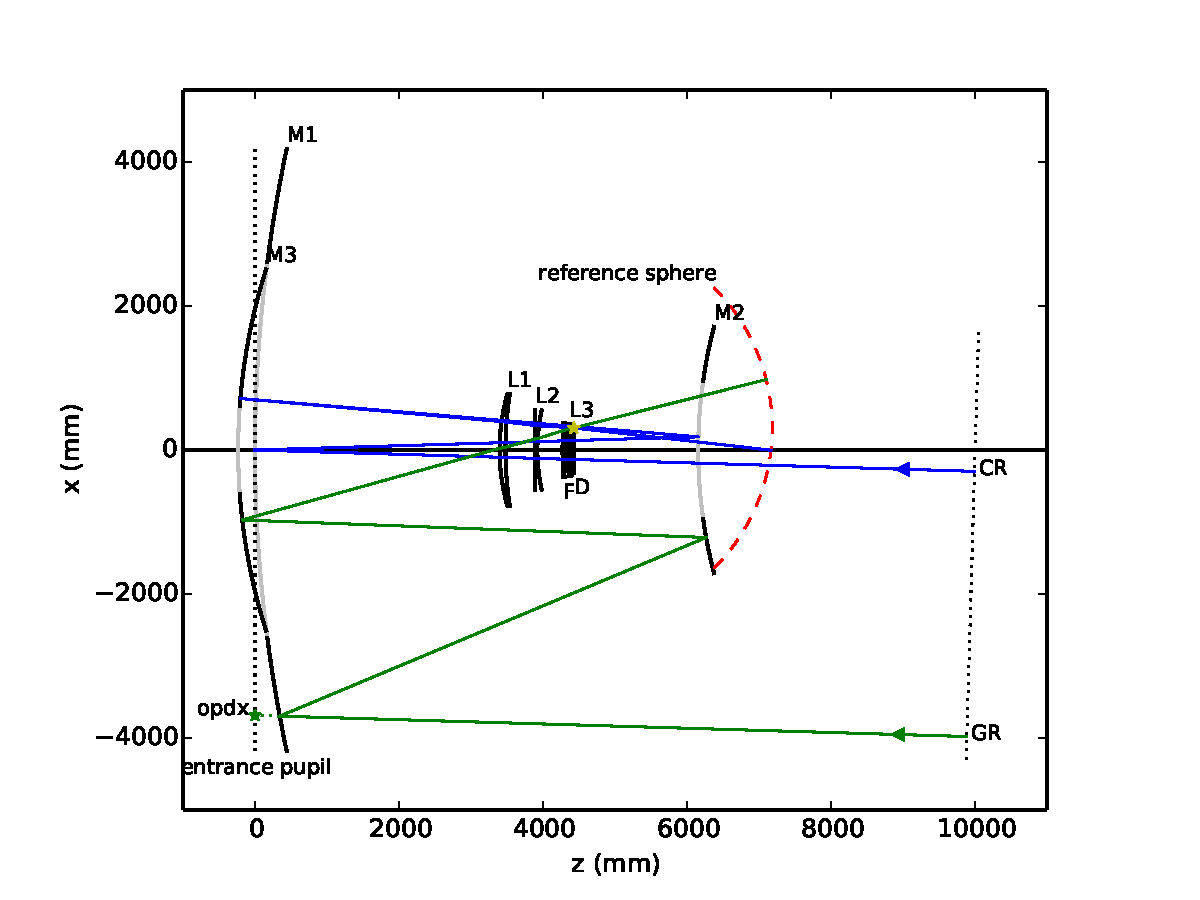
\includegraphics[width=6.0in]{layout.pdf}
\end{center}
\caption{LSST Layout}
\label{fig:layout}
\end{figure}
 

\section{Comparison with Zemax OPD}
Figure \ref{fig:opdmap} shows a PhoSim OPD map compared with Zemax's for a wavelength of 770 nm, 1.7$^{\circ}$ off-axis source without perturbation. The agreement between PhoSim and Zemax OPDs is at sub-nanometer scale. This numerical accuracy is achieved by setting \texttt{SURFACE\_POINTS} parameter to $10^5$ and \texttt{RAYTRACE\_TOLERANCE} parameter\footnote{Both are in \url{source/raytrace/parameter.h}. Default values of \texttt{SURFACE\_POINTS} and \texttt{RAYTRACE\_TOLERANCE} are 1024 and $10^{-6}$, respectively.} to $10^{-7}$. An higher accuracy is possible to achieved at the expense of computational time and memory.

\begin{figure}[h!tb]
%trim option's parameter order: left bottom right top
\begin{center}
\includegraphics[trim = 1cm 1cm 2cm 0cm, clip, width=6.5in]{opdmap.pdf}
\end{center}
\caption{OPD maps. {\it Upper left}: PhoSim OPD in wave numbers. {\it Upper right}: Zemax OPD in wave numbers. {\it Lower left}: difference between PhoSim and Zemax OPDs in nm. {\it Lower right}: fractional difference between PhoSim and Zemax OPDs.}
\label{fig:opdmap}
\end{figure}









\clearpage
\bibliographystyle{apj}
\bibliography{paper}

\end{document}
